% ============================================================================
% Authentication Implementation Documentation
% ============================================================================

\subsection{การออกแบบและ Implementation ระบบ Authentication}

ระบบ Authentication ถูกพัฒนาบน Rust Actix-Web โดยใช้หลักการ Clean Architecture แบ่งออกเป็น 4 Layer หลัก ได้แก่ Handler, Service, Repository และ Model โดยใช้ DTO (Data Transfer Object) เป็นตัวกลางในการรับส่งข้อมูลระหว่าง Layer

% ----------------------------------------------------------------------------
\subsubsection{Security Standards Reference}

การออกแบบระบบ Authentication อ้างอิงตามมาตรฐานความปลอดภัยระดับสากล:

\begin{table}[h]
\centering
\caption{มาตรฐานอ้างอิงสำหรับ Authentication}
\begin{tabular}{|p{3.5cm}|p{4cm}|p{6cm}|}
\hline
\textbf{มาตรฐาน} & \textbf{หมวด} & \textbf{การนำไปใช้} \\
\hline
OWASP ASVS V2 & Authentication & กำหนดแนวทาง password hashing, session management, และ credential storage \\
\hline
OWASP ASVS V2.4 & Credential Storage & กำหนดการใช้ memory-hard function (Argon2id) สำหรับ password hashing \\
\hline
OWASP Password Storage Cheat Sheet & Best Practices & กำหนด parameters สำหรับ Argon2id (memory, time, parallelism) \\
\hline
IETF RFC 9106 & Argon2 & มาตรฐาน Argon2 Password Hashing Function \\
\hline
IETF RFC 8446 & TLS 1.3 & มาตรฐานการเข้ารหัส Transport Layer สำหรับ API communication \\
\hline
PASETO Spec & Token Security & กำหนด V4 Local token format (XChaCha20-Poly1305) \\
\hline
\end{tabular}
\end{table}

\paragraph{OWASP ASVS V2 Requirements ที่ปฏิบัติตาม}~\\
\begin{itemize}
    \item \textbf{V2.4.1}: ใช้ password hashing function ที่ออกแบบมาสำหรับ password (Argon2id)
    \item \textbf{V2.4.2}: Salt มีความยาวอย่างน้อย 16 bytes และ unique ต่อทุก password
    \item \textbf{V2.4.3}: ใช้ sufficient work factors เพื่อให้ hash ใช้เวลาอย่างน้อย 1 วินาที
    \item \textbf{V2.1.1}: Credentials ไม่ถูก log หรือ expose ผ่าน error messages
    \item \textbf{V2.1.5}: Password verification ใช้ constant-time comparison
\end{itemize}

\paragraph{IETF RFC 9106 Compliance}~\\
Argon2id implementation ของระบบเป็นไปตาม \textbf{RFC 9106 (Argon2 Memory-Hard Function for Password Hashing)}:
\begin{itemize}
    \item ใช้ Argon2id variant (Section 4) ซึ่งรวมความปลอดภัยของทั้ง Argon2i และ Argon2d
    \item Salt generation ใช้ cryptographically secure random (Section 3.1)
    \item Output hash เป็น PHC string format ตาม Section 3
\end{itemize}

\clearpage

% ----------------------------------------------------------------------------
\subsubsection{Crates ที่ใช้งานและหน้าที่}

\begin{table}[h]
\centering
\caption{Crates สำหรับ Authentication}
\begin{tabular}{|p{3.5cm}|p{2cm}|p{8cm}|}
\hline
\textbf{Crate} & \textbf{Version} & \textbf{หน้าที่และคุณสมบัติ} \\
\hline
\texttt{argon2} & 0.5 & Password hashing algorithm ที่ได้รับรางวัล PHC (Password Hashing Competition) รองรับ Argon2id variant สำหรับป้องกันทั้ง side-channel และ GPU attacks \\
\hline
\texttt{rusty\_paseto} & 0.6 & PASETO (Platform-Agnostic Security Tokens) token library สำหรับสร้าง access และ refresh tokens แบบ V4 Local (symmetric encryption) \\
\hline
\texttt{secrecy} & 0.8 & Wrapper type สำหรับ sensitive data เช่น secret keys โดยป้องกันการ leak ผ่าน Debug traits และ logging \\
\hline
\texttt{validator} & 0.20 & Input validation library รองรับ derive macro สำหรับ validate fields เช่น length, email, range \\
\hline
\texttt{sqlx} & 0.8.6 & Async SQL toolkit รองรับ compile-time checked queries และ connection pooling แบบ async \\
\hline
\texttt{utoipa} & 5.4 & OpenAPI (Swagger) documentation generator แบบ automatic จาก code annotations \\
\hline
\end{tabular}
\end{table}

\clearpage

% ----------------------------------------------------------------------------
\subsubsection{Algorithms และ Cryptographic Primitives}

\paragraph{Argon2id Password Hashing}~\\
Argon2id เป็น hybrid variant ที่รวมข้อดีของ Argon2i (ป้องกัน side-channel attacks) และ Argon2d (ป้องกัน GPU cracking) โดยมี parameters หลัก 3 ตัว:

\begin{itemize}
    \item \textbf{Memory cost (m)}: จำนวน memory ที่ใช้ในการ hash (default: 19 MiB)
    \item \textbf{Time cost (t)}: จำนวน iterations (default: 2)
    \item \textbf{Parallelism (p)}: จำนวน threads ที่ใช้ (default: 1)
\end{itemize}

\begin{lstlisting}[language=Rust, caption=Password Hashing Implementation]
fn hash_password(password: &str) -> Result<String, AuthError> {
    let salt = SaltString::generate(&mut OsRng);
    let argon2 = Argon2::default(); // Argon2id with default parameters
    
    let password_hash = argon2
        .hash_password(password.as_bytes(), &salt)
        .map_err(|e| AuthError::HashingError(e.to_string()))?
        .to_string();
    
    Ok(password_hash)
}
\end{lstlisting}

\clearpage

\paragraph{PASETO V4 Local Token}~\\
PASETO (Platform-Agnostic Security Token) เป็น secure-by-default alternative ของ JWT โดย V4 Local ใช้:
\begin{itemize}
    \item \textbf{Encryption}: XChaCha20-Poly1305 (AEAD)
    \item \textbf{Key size}: 256-bit symmetric key
    \item \textbf{Nonce}: 192-bit random nonce
\end{itemize}

\begin{lstlisting}[language=Rust, caption=PASETO Token Generation]
fn generate_tokens(user: &User, config: &JwtConfig) 
    -> Result<(String, String), AuthError> {
    
    let key_bytes: [u8; 32] = /* 32-byte symmetric key */;
    let key = PasetoSymmetricKey::<V4, Local>::from(Key::from(key_bytes));
    
    // Access token (short-lived)
    let access_token = PasetoBuilder::<V4, Local>::default()
        .set_claim(ExpirationClaim::try_from(exp_str).unwrap())
        .set_claim(SubjectClaim::from(user_id_str))
        .set_claim(CustomClaim::try_from(("role", role_str)).unwrap())
        .build(&key)?;
    
    // Refresh token (long-lived - 7 days)
    let refresh_token = PasetoBuilder::<V4, Local>::default()
        .set_claim(ExpirationClaim::try_from(refresh_exp_str).unwrap())
        .set_claim(SubjectClaim::from(user_id_str))
        .build(&key)?;
    
    Ok((access_token, refresh_token))
}
\end{lstlisting}

% ----------------------------------------------------------------------------
\subsubsection{Complexity Analysis (Big O Notation)}

\begin{table}[h]
\centering
\caption{Time Complexity Analysis ของ Authentication Operations}
\begin{tabular}{|p{4cm}|p{2.5cm}|p{7cm}|}
\hline
\textbf{Operation} & \textbf{Time Complexity} & \textbf{Explanation} \\
\hline
Password Hashing (Argon2id) & $O(m \times t)$ & โดยที่ $m$ = memory blocks, $t$ = iterations; deliberately slow เพื่อป้องกัน brute-force \\
\hline
Password Verification & $O(m \times t)$ & ใช้ constant-time comparison เพื่อป้องกัน timing attacks \\
\hline
PASETO Token Generation & $O(n)$ & โดยที่ $n$ = payload size; XChaCha20 encryption เป็น linear time \\
\hline
Username Lookup (DB) & $O(\log n)$ & ใช้ B-Tree index บน username column \\
\hline
User Creation (DB) & $O(\log n)$ & INSERT with index maintenance \\
\hline
Input Validation & $O(k)$ & โดยที่ $k$ = จำนวน fields ที่ต้อง validate; linear scan \\
\hline
\end{tabular}
\end{table}

\paragraph{Space Complexity}~\\
\begin{itemize}
    \item \textbf{Argon2id}: $O(m)$ โดยที่ $m$ คือ memory cost parameter (default 19 MiB)
    \item \textbf{PASETO Token}: $O(n)$ โดยที่ $n$ คือขนาดของ claims ที่ embed ใน token
    \item \textbf{Database Connection Pool}: $O(c)$ โดยที่ $c$ คือจำนวน max connections
\end{itemize}

\clearpage

% ----------------------------------------------------------------------------
\subsubsection{Data Structures และ DTOs}

\paragraph{Model Layer}~\\
\texttt{User} model ถูกออกแบบให้ map กับ \texttt{users} table โดยตรง:

\begin{lstlisting}[language=Rust, caption=User Model Structure]
#[derive(Debug, Clone, FromRow, Serialize, Deserialize)]
pub struct User {
    pub user_id: Uuid,          // Primary key (UUID v4)
    pub username: String,        // Unique constraint
    pub password_hash: String,   // Argon2id hash
    pub role: UserRole,          // Enum: Researcher | Student | Lecturer
    pub created_at: Option<DateTime<Utc>>,
}

#[derive(Debug, Clone, Copy, PartialEq, Eq, sqlx::Type)]
#[sqlx(type_name = "user_role", rename_all = "lowercase")]
pub enum UserRole {
    Researcher,
    Student,
    Lecturer,
}
\end{lstlisting}

\paragraph{DTO (Data Transfer Objects)}~\\
DTOs แยกระหว่าง Request และ Response เพื่อควบคุม data exposure:

\begin{lstlisting}[language=Rust, caption=Authentication DTOs]
// Request DTOs with validation
#[derive(Debug, Deserialize, Validate, ToSchema)]
pub struct RegisterRequest {
    #[validate(length(min = 3, max = 255))]
    pub username: String,
    #[validate(length(min = 8))]
    pub password: String,
    pub role: Option<UserRole>,  // Default: Student
}

#[derive(Debug, Deserialize, Validate, ToSchema)]
pub struct LoginRequest {
    #[validate(length(min = 1))]
    pub username: String,
    #[validate(length(min = 1))]
    pub password: String,
}

// Response DTOs (no sensitive data)
#[derive(Debug, Serialize, ToSchema)]
pub struct LoginResponse {
    pub access_token: String,
    pub refresh_token: String,
    pub expires_in: i64,         // Seconds until expiration
    pub user: UserResponse,
}

#[derive(Debug, Serialize, ToSchema)]
pub struct UserResponse {
    pub user_id: Uuid,
    pub username: String,
    pub role: String,            // No password_hash exposed
}
\end{lstlisting}

\paragraph{API Response Wrapper}~\\
ทุก API response ถูก wrap ด้วย \texttt{ApiResponse<T>} เพื่อความ consistency:

\begin{lstlisting}[language=Rust, caption=Standard API Response Wrapper]
#[derive(Debug, Serialize, ToSchema)]
pub struct ApiResponse<T: Serialize> {
    pub success: bool,
    #[serde(skip_serializing_if = "Option::is_none")]
    pub data: Option<T>,
    #[serde(skip_serializing_if = "Option::is_none")]
    pub error: Option<ApiError>,
}

#[derive(Debug, Serialize, ToSchema)]
pub struct ApiError {
    pub code: String,      // e.g., "INVALID_CREDENTIALS"
    pub message: String,   // Human-readable message
}
\end{lstlisting}

% ----------------------------------------------------------------------------
\subsubsection{Repository Pattern}

Repository layer encapsulate database queries โดยใช้ \texttt{sqlx} compile-time checked queries:

\begin{lstlisting}[language=Rust, caption=User Repository Implementation]
pub struct UserRepository;

impl UserRepository {
    /// Create user: O(log n) with index maintenance
    pub async fn create(pool: &PgPool, username: &str, 
                        password_hash: &str, role: UserRole) 
        -> Result<User, sqlx::Error> {
        sqlx::query_as::<_, User>(r#"
            INSERT INTO users (username, password_hash, role)
            VALUES ($1, $2, $3)
            RETURNING user_id, username, password_hash, role, created_at
        "#)
        .bind(username).bind(password_hash).bind(role)
        .fetch_one(pool).await
    }
    
    /// Find by username: O(log n) using B-Tree index
    pub async fn find_by_username(pool: &PgPool, username: &str) 
        -> Result<Option<User>, sqlx::Error> {
        sqlx::query_as::<_, User>(r#"
            SELECT user_id, username, password_hash, role, created_at
            FROM users WHERE username = $1
        "#)
        .bind(username)
        .fetch_optional(pool).await
    }
    
    /// Check existence: O(log n) with EXISTS subquery
    pub async fn username_exists(pool: &PgPool, username: &str) 
        -> Result<bool, sqlx::Error> {
        sqlx::query_scalar::<_, bool>(r#"
            SELECT EXISTS(SELECT 1 FROM users WHERE username = $1)
        "#)
        .bind(username)
        .fetch_one(pool).await
    }
}
\end{lstlisting}

% ----------------------------------------------------------------------------
\subsubsection{Authentication Flow}

\paragraph{Registration Flow}~\\
\begin{enumerate}
    \item Handler รับ \texttt{RegisterRequest} และ validate input
    \item Service ตรวจสอบ username uniqueness ผ่าน Repository
    \item Service hash password ด้วย Argon2id
    \item Repository บันทึก user ลง database
    \item ส่ง \texttt{RegisterResponse} กลับ (ไม่มี password hash)
\end{enumerate}

\paragraph{Login Flow}~\\
\begin{enumerate}
    \item Handler รับ \texttt{LoginRequest} และ validate input
    \item Service ค้นหา user จาก username ผ่าน Repository
    \item Service verify password กับ stored hash (constant-time comparison)
    \item Service generate PASETO tokens (access + refresh)
    \item ส่ง \texttt{LoginResponse} พร้อม tokens และ user info
\end{enumerate}

\begin{figure}[h]
\centering
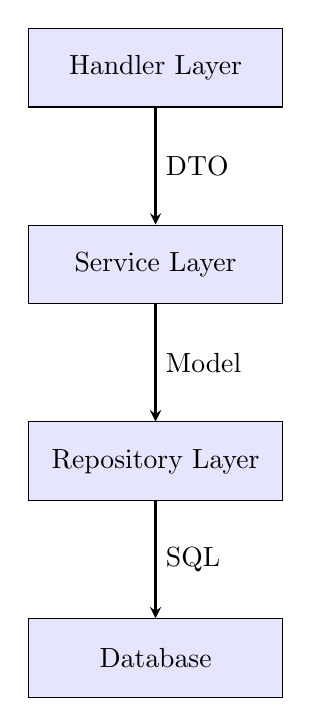
\begin{tikzpicture}[node distance=2.5cm, auto]
    % Styles
    \tikzstyle{layer} = [rectangle, draw, fill=blue!10, text width=3cm, text centered, minimum height=1cm]
    \tikzstyle{arrow} = [thick, ->, >=stealth]
    
    % Nodes
    \node[layer] (handler) {Handler Layer};
    \node[layer, below of=handler] (service) {Service Layer};
    \node[layer, below of=service] (repo) {Repository Layer};
    \node[layer, below of=repo] (db) {Database};
    
    % Arrows
    \draw[arrow] (handler) -- node[right] {DTO} (service);
    \draw[arrow] (service) -- node[right] {Model} (repo);
    \draw[arrow] (repo) -- node[right] {SQL} (db);
\end{tikzpicture}
\caption{Authentication Layer Architecture}
\end{figure}

% ----------------------------------------------------------------------------
\subsubsection{Error Handling}

ระบบใช้ \texttt{thiserror} crate สำหรับ structured error handling:

\begin{lstlisting}[language=Rust, caption=Authentication Error Types]
#[derive(Debug, Error)]
pub enum AuthError {
    #[error("Username already exists")]
    UsernameExists,

    #[error("Invalid credentials")]
    InvalidCredentials,

    #[error("Password hashing failed: {0}")]
    HashingError(String),

    #[error("Token generation failed: {0}")]
    TokenError(String),

    #[error("Database error: {0}")]
    DatabaseError(#[from] sqlx::Error),

    #[error("Validation error: {0}")]
    ValidationError(String),
}
\end{lstlisting}

\begin{table}[h]
\centering
\caption{HTTP Status Code Mapping}
\begin{tabular}{|l|l|l|}
\hline
\textbf{AuthError} & \textbf{HTTP Status} & \textbf{Error Code} \\
\hline
\texttt{UsernameExists} & 409 Conflict & \texttt{USERNAME\_EXISTS} \\
\hline
\texttt{InvalidCredentials} & 401 Unauthorized & \texttt{INVALID\_CREDENTIALS} \\
\hline
\texttt{ValidationError} & 400 Bad Request & \texttt{VALIDATION\_ERROR} \\
\hline
\texttt{DatabaseError} & 500 Internal Server Error & \texttt{INTERNAL\_ERROR} \\
\hline
\end{tabular}
\end{table}

% ----------------------------------------------------------------------------
\subsubsection{Security Considerations}

\begin{itemize}
    \item \textbf{Password Storage}: ใช้ Argon2id ซึ่งเป็น memory-hard function ป้องกัน GPU/ASIC attacks
    \item \textbf{Constant-time Comparison}: Password verification ใช้ constant-time comparison เพื่อป้องกัน timing attacks
    \item \textbf{Secret Management}: ใช้ \texttt{secrecy} crate ป้องกัน secret keys จากการ leak ผ่าน logs
    \item \textbf{Token Design}: PASETO เป็น secure-by-default ไม่มี algorithm negotiation vulnerabilities เหมือน JWT
    \item \textbf{No Password in Response}: Response DTOs ไม่มี password\_hash field ป้องกัน accidental exposure
    \item \textbf{Input Validation}: ทุก request ผ่าน validation ก่อน processing
\end{itemize}

% ----------------------------------------------------------------------------
\subsubsection{Logout Flow}

\paragraph{Stateless Logout Strategy}~\\
ระบบนี้ใช้ stateless authentication โดย PASETO tokens ไม่ถูกเก็บใน database ดังนั้น logout จึงเป็นการบอก client ให้ลบ tokens ออกจาก storage (localStorage, sessionStorage, หรือ cookie)

\paragraph{Logout Flow}~\\
\begin{enumerate}
    \item Client ส่ง POST request ไปที่ \texttt{/api/v1/auth/logout} พร้อม Bearer token
    \item AuthenticationMiddleware validate token (ตรวจสอบว่า user ยัง authenticated อยู่)
    \item Handler คืน response บอกว่า logout สำเร็จ
    \item Client ลบ access\_token และ refresh\_token ออกจาก storage
\end{enumerate}

\begin{lstlisting}[language=Rust, caption=Logout Handler Implementation]
/// Logout user (Stateless)
#[utoipa::path(
    post,
    path = "/api/v1/auth/logout",
    tag = "Authentication",
    security(("bearer_auth" = [])),
    responses(
        (status = 200, description = "Logout successful"),
        (status = 401, description = "Unauthorized")
    )
)]
pub async fn logout() -> HttpResponse {
    HttpResponse::Ok().json(ApiResponse::success(LogoutResponse {
        message: "Logged out successfully. Please discard your tokens.".to_string(),
    }))
}
\end{lstlisting}

\paragraph{LogoutResponse DTO}~\\
\begin{lstlisting}[language=Rust, caption=Logout Response Structure]
#[derive(Debug, Clone, Serialize, ToSchema)]
pub struct LogoutResponse {
    pub message: String,
}

// Example response:
{
    "success": true,
    "data": {
        "message": "Logged out successfully. Please discard your tokens."
    }
}
\end{lstlisting}

\paragraph{Security Note}~\\
\begin{itemize}
    \item \textbf{Token Invalidation}: เนื่องจากเป็น stateless ระบบไม่สามารถ invalidate token จาก server-side ได้ทันที
    \item \textbf{Short-lived Tokens}: Access token ถูกตั้งมี expiration time สั้น (เช่น 15 นาที) เพื่อลด window of vulnerability
    \item \textbf{Refresh Token Rotation}: หาก implement token revocation ในอนาคต ควรเก็บ refresh token ใน database และลบตอน logout
\end{itemize}
